\section{Differential Functions on a regular surface}
\begin{question}[1]
    How to define a function on $\mathbb{S}^2$?
\end{question}
In calculus, we have seen this is just $f\left(x,y,z
    \right)|_{\mathbb{S}^2}$, but what does this mean?
If $p\in $ upper half semi-sphere $\Rightarrow$ $f\left(x,y,\sqrt{1-x^2-y^2}\right)$ $\Rightarrow f$ is just a function on
\[
    U={(x,y)\in \mathbb{R}^3\colon x^2+y^2<1}  .
\]

More precisely, if we let $F\colon U\to \mathbb{S}^2$ be the local parametrization,
\[
    (x,y)\mapsto (x,y,\sqrt{1-x^2-y^2}),
\]
then $\tilde{f}(x,y)\colon U\to \mathbb{R}, \tilde{f}(x,y)=f\circ  F$.

Similarly, if the point lies on other five charts(see \cref{charts on unit sphere}). There is also a function $\tilde{f}$ essentially defined on an open set of $\mathbb{R}^2$ to associate $f$.

\begin{question}[2]
    What does it mean by a ``smooth'' (or differentiable) function on $\mathbb{S}^2$?
\end{question}
\begin{align*}
    f \text{ is smooth near }p \Leftrightarrow &
    \tilde{f}\colon U\subset \mathbb{R}^2 \to \mathbb{R} \text{is smooth,}                                                 \\
                                               & (\because F\colon U\subset \mathbb{R}^2\to \mathbb{S}^2 \text{is smooth})
\end{align*}
\begin{question}[3]
    $p$ could lie on two charts, (\ie\ we can associate two coordinate charts near $p$, will the ``smoothness'' of $f$ be affected?)
\end{question}

\tikzset{every picture/.style={line width=0.75pt}} %set default line width to 0.75pt        

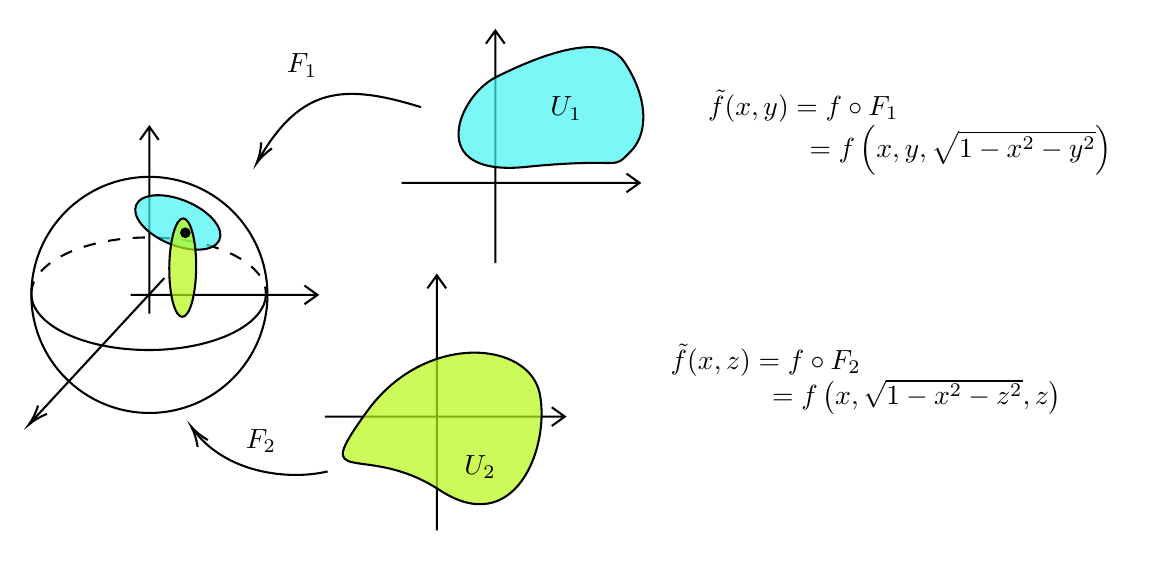
\begin{tikzpicture}[x=0.75pt,y=0.75pt,yscale=-0.9,xscale=0.9]
    %uncomment if require: \path (0,300); %set diagram left start at 0, and has height of 300

    %Shape: Axis 2D [id:dp5905610283034792] 
    \draw  (128,153) -- (228,153)(138,63) -- (138,163) (221,148) -- (228,153) -- (221,158) (133,70) -- (138,63) -- (143,70)  ;
    %Straight Lines [id:da5258527733857374] 
    \draw    (146,144) -- (74.76,221.03) ;
    \draw [shift={(73.4,222.5)}, rotate = 312.76] [color={rgb, 255:red, 0; green, 0; blue, 0 }  ][line width=0.75]    (10.93,-3.29) .. controls (6.95,-1.4) and (3.31,-0.3) .. (0,0) .. controls (3.31,0.3) and (6.95,1.4) .. (10.93,3.29)   ;
    %Shape: Circle [id:dp7596976921705518] 
    \draw   (74.8,153) .. controls (74.8,118.1) and (103.1,89.8) .. (138,89.8) .. controls (172.9,89.8) and (201.2,118.1) .. (201.2,153) .. controls (201.2,187.9) and (172.9,216.2) .. (138,216.2) .. controls (103.1,216.2) and (74.8,187.9) .. (74.8,153) -- cycle ;
    %Shape: Arc [id:dp4458065415749495] 
    \draw  [draw opacity=0] (200.4,152.37) .. controls (200.4,152.37) and (200.4,152.37) .. (200.4,152.37) .. controls (200.4,169.01) and (172.28,182.5) .. (137.6,182.5) .. controls (102.92,182.5) and (74.8,169.01) .. (74.8,152.37) -- (137.6,152.37) -- cycle ; \draw   (200.4,152.37) .. controls (200.4,152.37) and (200.4,152.37) .. (200.4,152.37) .. controls (200.4,169.01) and (172.28,182.5) .. (137.6,182.5) .. controls (102.92,182.5) and (74.8,169.01) .. (74.8,152.37) ;
    %Shape: Arc [id:dp1079879229191647] 
    \draw  [draw opacity=0][dash pattern={on 4.5pt off 4.5pt}] (74.8,152.37) .. controls (74.8,152.37) and (74.8,152.37) .. (74.8,152.37) .. controls (74.8,135.74) and (102.92,122.25) .. (137.6,122.25) .. controls (172.28,122.25) and (200.4,135.74) .. (200.4,152.37) -- (137.6,152.37) -- cycle ; \draw  [dash pattern={on 4.5pt off 4.5pt}] (74.8,152.37) .. controls (74.8,152.37) and (74.8,152.37) .. (74.8,152.37) .. controls (74.8,135.74) and (102.92,122.25) .. (137.6,122.25) .. controls (172.28,122.25) and (200.4,135.74) .. (200.4,152.37) ;
    %Shape: Circle [id:dp8215567727809696] 
    \draw  [fill={rgb, 255:red, 67; green, 243; blue, 243 }  ,fill opacity=0.7 ] (136.48,118.05) .. controls (127.92,110.28) and (128.47,102.27) .. (137.71,100.15) .. controls (146.96,98.03) and (161.39,102.61) .. (169.95,110.38) .. controls (178.51,118.14) and (177.96,126.16) .. (168.71,128.27) .. controls (159.47,130.39) and (145.04,125.81) .. (136.48,118.05) -- cycle ;
    %Shape: Ellipse [id:dp5973540554680155] 
    \draw  [fill={rgb, 255:red, 182; green, 250; blue, 18 }  ,fill opacity=0.7 ] (153.21,114.21) .. controls (156.92,108.46) and (161.1,114.64) .. (162.55,128) .. controls (164.01,141.36) and (162.19,156.86) .. (158.49,162.6) .. controls (154.79,168.35) and (150.6,162.18) .. (149.15,148.81) .. controls (147.69,135.45) and (149.51,119.96) .. (153.21,114.21) -- cycle ;
    %Shape: Circle [id:dp24020151067783413] 
    \draw  [fill={rgb, 255:red, 0; green, 0; blue, 0 }  ,fill opacity=1 ] (155,119.75) .. controls (155,118.51) and (156.01,117.5) .. (157.25,117.5) .. controls (158.49,117.5) and (159.5,118.51) .. (159.5,119.75) .. controls (159.5,120.99) and (158.49,122) .. (157.25,122) .. controls (156.01,122) and (155,120.99) .. (155,119.75) -- cycle ;
    %Shape: Axis 2D [id:dp6541206749950883] 
    \draw  (273,93.05) -- (400.4,93.05)(323.2,11.5) -- (323.2,136) (393.4,88.05) -- (400.4,93.05) -- (393.4,98.05) (318.2,18.5) -- (323.2,11.5) -- (328.2,18.5)  ;
    %Shape: Polygon Curved [id:ds3396588391090478] 
    \draw  [fill={rgb, 255:red, 67; green, 243; blue, 243 }  ,fill opacity=0.7 ] (323.4,36.5) .. controls (343.4,26.5) and (380.4,10.5) .. (392.4,28.5) .. controls (394.54,31.71) and (396.35,34.97) .. (397.81,38.22) .. controls (404.56,53.16) and (404.05,67.85) .. (395.4,76.5) .. controls (386.1,85.8) and (391.98,80.62) .. (356.01,83.08) .. controls (351.25,83.4) and (345.76,83.86) .. (339.4,84.5) .. controls (285,90) and (303.4,46.5) .. (323.4,36.5) -- cycle ;
    %Shape: Axis 2D [id:dp15349087590497468] 
    \draw  (232,218.15) -- (360.4,218.15)(291.87,142.5) -- (291.87,279) (353.4,213.15) -- (360.4,218.15) -- (353.4,223.15) (286.87,149.5) -- (291.87,142.5) -- (296.87,149.5)  ;
    %Shape: Polygon Curved [id:ds9697525934649356] 
    \draw  [fill={rgb, 255:red, 182; green, 250; blue, 18 }  ,fill opacity=0.7 ] (254.4,215.5) .. controls (285.4,172.5) and (341.4,177.5) .. (347,206) .. controls (352.6,234.5) and (333.8,284) .. (293.4,257.5) .. controls (253,231) and (223.4,258.5) .. (254.4,215.5) -- cycle ;
    %Curve Lines [id:da20815011674520578] 
    \draw    (283.4,52.5) .. controls (241.82,39.63) and (218.86,41.46) .. (196.09,81.28) ;
    \draw [shift={(195.4,82.5)}, rotate = 299.29] [color={rgb, 255:red, 0; green, 0; blue, 0 }  ][line width=0.75]    (10.93,-3.29) .. controls (6.95,-1.4) and (3.31,-0.3) .. (0,0) .. controls (3.31,0.3) and (6.95,1.4) .. (10.93,3.29)   ;
    %Curve Lines [id:da056699720507130014] 
    \draw    (233.4,247.5) .. controls (212.82,252.4) and (178.79,248.66) .. (161.44,224.97) ;
    \draw [shift={(160.4,223.5)}, rotate = 55.78] [color={rgb, 255:red, 0; green, 0; blue, 0 }  ][line width=0.75]    (10.93,-3.29) .. controls (6.95,-1.4) and (3.31,-0.3) .. (0,0) .. controls (3.31,0.3) and (6.95,1.4) .. (10.93,3.29)   ;

    % Text Node
    \draw (428,41.4) node [anchor=north west][inner sep=0.75pt]    {$ \begin{array}{l}
                \tilde{f}( x,y) =f\circ F_{1} \\
                \ \ \ \ \ \ \ \ \ \ \ =f\left( x,y,\sqrt{1-x^{2} -y^{2}}\right)
            \end{array}$};
    % Text Node
    \draw (408,177.4) node [anchor=north west][inner sep=0.75pt]    {$ \begin{array}{l}
                \tilde{f}( x,z) =f\circ F_{2} \\
                \ \ \ \ \ \ \ \ \ \ \ =f\left( x,\sqrt{1-x^{2} -z^{2}} ,z\right)
            \end{array}$};
    % Text Node
    \draw (210,22.4) node [anchor=north west][inner sep=0.75pt]    {$F_{1}$};
    % Text Node
    \draw (188,223.4) node [anchor=north west][inner sep=0.75pt]    {$F_{2}$};
    % Text Node
    \draw (351,45.4) node [anchor=north west][inner sep=0.75pt]    {$U_{1}$};
    % Text Node
    \draw (305,237.4) node [anchor=north west][inner sep=0.75pt]    {$U_{2}$};


\end{tikzpicture}

Smoothness is not affected by the coordinate change. Moreover, it's easy to
apply the chain rule to find relation of differentials of f between
different coordinate charts.
\begin{definition}[Differential function]
    $S$ is a regular surface in $\mathbb{R}^3$. A function $f$ is said to
    be differentiable at $p\in S$, if for a local parametrization near $p$
    \[
        x\colon U\subset \mathbb{R}^2\to \mathbb{R}^3,
    \]
    the function $f\circ x\colon \mathbb{R}^2\to \mathbb{R}$ is
    differentiable at $x^{-1}(p)$
\end{definition}
\begin{remark}
    $f\circ x$ is well-defined, since the differentiability is not affected
    by a change of parameter, e.g. if $y\colon V\subset \mathbb{R}^2\to\
        mathbb{R}^3$ is another parametrization near $p$, $f\circ y=f\circ
        x\circ(\underbrace{x^{-1}\circ y}_{\text{change of parameter}})$ is
    differentiable.
\end{remark}
\begin{example}
    Consider $x^2+y^2+(z-1)^2$=1.
    \begin{enumerate}[(1)]
        \item  Consider $\va{X}=(x,y,z)$ be the position vector field in
              $\mathbb{R}^3$. Let $f(x,y,z)=\va{X}\vdot \va{n}$
              where $\va{n}=(0,0,1)$ is the unit normal of $xy$
              plane.
              \begin{center}



                  \tikzset{every picture/.style={line width=0.75pt}} %set default line width to 0.75pt        

                  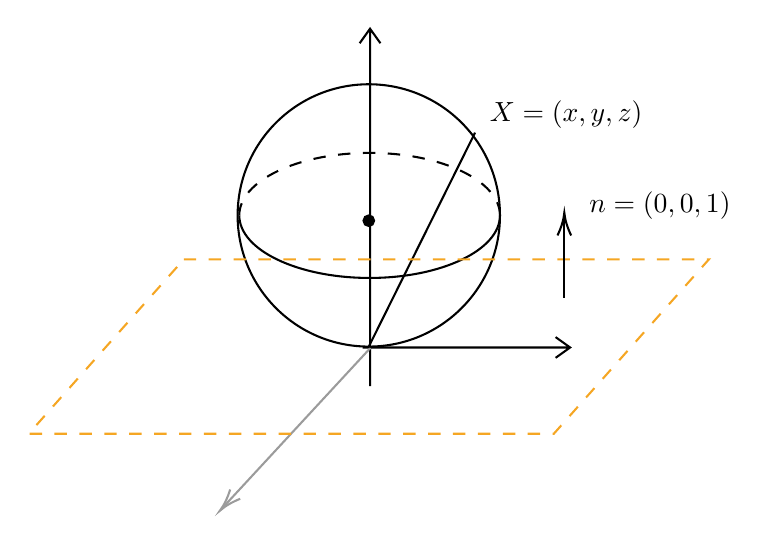
\begin{tikzpicture}[x=0.75pt,y=0.75pt,yscale=-1,xscale=1]
                      %uncomment if require: \path (0,300); %set diagram left start at 0, and has height of 300

                      %Shape: Axis 2D [id:dp5905610283034792] 
                      \draw  (299.2,197) -- (399.2,197)(302.8,43.42) -- (302.8,215.62) (392.2,192) -- (399.2,197) -- (392.2,202) (297.8,50.42) -- (302.8,43.42) -- (307.8,50.42)  ;
                      %Straight Lines [id:da5258527733857374] 
                      \draw [color={rgb, 255:red, 155; green, 155; blue, 155 }  ,draw opacity=1 ]   (303,197.2) -- (260.68,242.96) -- (231.76,274.23) ;
                      \draw [shift={(230.4,275.7)}, rotate = 312.76] [color={rgb, 255:red, 155; green, 155; blue, 155 }  ,draw opacity=1 ][line width=0.75]    (10.93,-3.29) .. controls (6.95,-1.4) and (3.31,-0.3) .. (0,0) .. controls (3.31,0.3) and (6.95,1.4) .. (10.93,3.29)   ;
                      %Shape: Circle [id:dp7596976921705518] 
                      \draw   (239,133.37) .. controls (239,98.47) and (267.3,70.18) .. (302.2,70.18) .. controls (337.1,70.18) and (365.4,98.47) .. (365.4,133.37) .. controls (365.4,168.28) and (337.1,196.57) .. (302.2,196.57) .. controls (267.3,196.57) and (239,168.28) .. (239,133.37) -- cycle ;
                      %Shape: Arc [id:dp4458065415749495] 
                      \draw  [draw opacity=0] (365.4,133.37) .. controls (365.4,150.01) and (337.28,163.5) .. (302.6,163.5) .. controls (267.92,163.5) and (239.8,150.01) .. (239.8,133.37) -- (302.6,133.37) -- cycle ; \draw   (365.4,133.37) .. controls (365.4,150.01) and (337.28,163.5) .. (302.6,163.5) .. controls (267.92,163.5) and (239.8,150.01) .. (239.8,133.37) ;
                      %Shape: Arc [id:dp1079879229191647] 
                      \draw  [draw opacity=0][dash pattern={on 4.5pt off 4.5pt}] (239.8,133.37) .. controls (239.8,116.74) and (267.92,103.25) .. (302.6,103.25) .. controls (337.28,103.25) and (365.4,116.74) .. (365.4,133.37) -- (302.6,133.37) -- cycle ; \draw  [dash pattern={on 4.5pt off 4.5pt}] (239.8,133.37) .. controls (239.8,116.74) and (267.92,103.25) .. (302.6,103.25) .. controls (337.28,103.25) and (365.4,116.74) .. (365.4,133.37) ;
                      %Straight Lines [id:da4102003893399948] 
                      \draw    (353.4,93.5) -- (302.2,196.57) ;
                      %Shape: Circle [id:dp09109443249657256] 
                      \draw  [color={rgb, 255:red, 0; green, 0; blue, 0 }  ,draw opacity=1 ][fill={rgb, 255:red, 0; green, 0; blue, 0 }  ,fill opacity=1 ] (299.65,135.92) .. controls (299.65,134.52) and (300.79,133.37) .. (302.2,133.37) .. controls (303.61,133.37) and (304.75,134.52) .. (304.75,135.92) .. controls (304.75,137.33) and (303.61,138.47) .. (302.2,138.47) .. controls (300.79,138.47) and (299.65,137.33) .. (299.65,135.92) -- cycle ;
                      %Shape: Parallelogram [id:dp22036772290852347] 
                      \draw  [color={rgb, 255:red, 245; green, 166; blue, 35 }  ,draw opacity=1 ][dash pattern={on 4.5pt off 4.5pt}] (213.05,154.57) -- (466.05,154.57) -- (391.35,238.57) -- (138.35,238.57) -- cycle ;
                      %Straight Lines [id:da5141552556306255] 
                      \draw    (396.4,173.1) -- (396.4,134.1) ;
                      \draw [shift={(396.4,132.1)}, rotate = 90] [color={rgb, 255:red, 0; green, 0; blue, 0 }  ][line width=0.75]    (10.93,-3.29) .. controls (6.95,-1.4) and (3.31,-0.3) .. (0,0) .. controls (3.31,0.3) and (6.95,1.4) .. (10.93,3.29)   ;

                      % Text Node
                      \draw (359,76.4) node [anchor=north west][inner sep=0.75pt]    {$\va{X}=( x,y,z)$};
                      % Text Node
                      \draw (407,120.4) node [anchor=north west][inner sep=0.75pt]    {$\va{n} =( 0,0,1)$};


                  \end{tikzpicture}
              \end{center}
              $\Rightarrow f(x,y,z)=z$.
              At point $(x,y,z)\in \mathbb{S^2},\quad z>1$,
              $f(x,y,z)=1+\sqrt{1-x^2-y^2}$, where $x^2+y^2<1$,
              it's a smooth function.
        \item Consider $d^2(x,y,z)=x^2+y^2+z^2=|\va{X}|
                  ^2$, d
              is the distance function on $\mathbb{R}^2$. $d^2|_
                  {\mathbb{S}^2}=2 z= 2f$ in (1), hence it's a smooth
              function.
    \end{enumerate}
\end{example}
\begin{exercise}
    How does the function $f$ look like in other
    coordinate charts?
\end{exercise}
\begin{definition}[Differentiable mapping between two surfaces]
    $S_1,S_2$ are regular surfaces, $\varphi\colon S_1\to
        S_2$ is a mapping that maps $p\in S_1$ to $\varphi(p)
        \in S_2$. We say $\varphi$ is differentiable at $p\in
        S$, if for some parametrization
    \[
        F\colon U_1\to S_1(\ni p),\quad F_2\colon U_2
        \to S_2(\ni \varphi(p))
    \]
    \[
        F_2^{-1}\circ \varphi \circ F_1\colon U_1\to U_2
        \text{ is differentiable at }F_1^{-1}(p).
    \]
    \begin{center}



        \tikzset{every picture/.style={line width=0.75pt}} %set default line width to 0.75pt        

        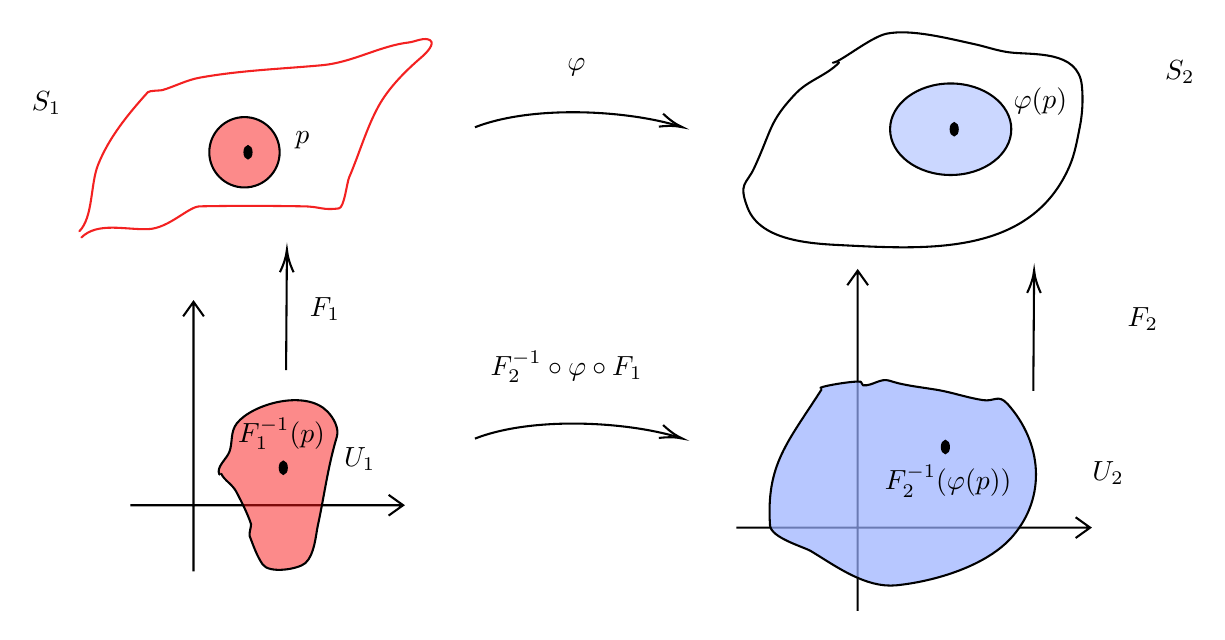
\begin{tikzpicture}[x=0.75pt,y=0.75pt,yscale=-1,xscale=1]
            %uncomment if require: \path (0,300); %set diagram left start at 0, and has height of 300

            %Shape: Axis 2D [id:dp3168627496867378] 
            \draw  (118,241.1) -- (249.4,241.1)(148.4,143.1) -- (148.4,273) (242.4,236.1) -- (249.4,241.1) -- (242.4,246.1) (143.4,150.1) -- (148.4,143.1) -- (153.4,150.1)  ;
            %Curve Lines [id:da7660218913325227] 
            \draw [fill={rgb, 255:red, 250; green, 21; blue, 21 }  ,fill opacity=0.5 ][line width=0.75] [line join = round][line cap = round]   (161.75,225.91) .. controls (163.21,229.11) and (167.16,231.03) .. (169.05,234.68) .. controls (171.65,239.71) and (174.3,244.77) .. (176.1,250.14) .. controls (176.37,250.96) and (175,254.77) .. (175.45,255.94) .. controls (177.24,260.61) and (178.88,265.44) .. (181.67,269.58) .. controls (184.83,274.26) and (198.97,271.92) .. (202.28,268.98) .. controls (206.76,265) and (207.31,255.37) .. (208.3,250.85) .. controls (210.41,241.18) and (211.84,231.78) .. (213.89,222.2) .. controls (214.88,217.6) and (216.01,212.95) .. (217.43,208.21) .. controls (218.67,204.05) and (215.96,199.1) .. (212.94,195.97) .. controls (202.48,185.12) and (176.92,192.17) .. (169.33,201.57) .. controls (166.02,205.68) and (167.34,210.96) .. (165.71,215.31) .. controls (164.35,218.95) and (159.15,222.63) .. (160.84,226.33) ;
            %Shape: Axis 2D [id:dp528543087337018] 
            \draw  (410,251.9) -- (580.4,251.9)(468.4,128.1) -- (468.4,292) (573.4,246.9) -- (580.4,251.9) -- (573.4,256.9) (463.4,135.1) -- (468.4,128.1) -- (473.4,135.1)  ;
            %Curve Lines [id:da3774751912241312] 
            \draw [fill={rgb, 255:red, 152; green, 175; blue, 255 }  ,fill opacity=0.7 ][line width=0.75] [line join = round][line cap = round]   (450.96,185.36) .. controls (434.61,210.92) and (424.22,221.45) .. (426.16,250.82) .. controls (426.55,256.8) and (442.57,261.22) .. (445.85,263.2) .. controls (457.8,270.39) and (472.24,281.19) .. (487.08,279.68) .. controls (505.36,277.82) and (530.67,270.45) .. (543.11,255.99) .. controls (559.48,236.96) and (557.22,210.87) .. (540.68,192.4) .. controls (536.12,187.31) and (534.36,191.29) .. (528.8,190.47) .. controls (521.34,189.36) and (514.15,186.78) .. (506.72,185.52) .. controls (505.84,185.38) and (504.96,185.23) .. (504.08,185.1) .. controls (497.07,184.01) and (489.7,183.15) .. (483.79,181.12) .. controls (479.39,179.6) and (475.39,183.81) .. (470.98,183.32) .. controls (470.32,183.25) and (470.56,181.78) .. (469.91,181.63) .. controls (467.04,180.99) and (451.91,183.57) .. (450.42,184.51) ;
            %Curve Lines [id:da0882085470935694] 
            \draw [color={rgb, 255:red, 243; green, 33; blue, 33 }  ,draw opacity=1 ][line width=0.75] [line join = round][line cap = round]   (93.4,109.1) .. controls (100.05,102.45) and (98.71,86.33) .. (102.4,77.1) .. controls (107.6,64.1) and (116.44,53.16) .. (126.4,42.1) .. controls (127.15,41.27) and (132.47,41.38) .. (133.4,41.1) .. controls (139.46,39.28) and (145.17,36.21) .. (151.4,35.1) .. controls (171.15,31.57) and (190.63,30.9) .. (210.4,29.1) .. controls (225.05,27.77) and (238.4,19.66) .. (252.4,18.1) .. controls (255.06,17.8) and (259.8,15.37) .. (262.4,17.1) .. controls (264.88,18.75) and (260.66,23.16) .. (258.4,25.1) .. controls (250.53,31.85) and (242.37,39.98) .. (237.4,49.1) .. controls (231.72,59.52) and (228.23,71.84) .. (223.4,83.1) .. controls (222.2,85.9) and (221.08,97.77) .. (218.4,98.1) .. controls (210.26,99.12) and (209.8,97.24) .. (201.4,97.1) .. controls (184.74,96.82) and (168.06,96.77) .. (151.4,97.1) .. controls (145.91,97.21) and (136.51,107.77) .. (126.4,108.1) .. controls (115.66,108.45) and (102,104.5) .. (94.4,112.1) ;
            %Shape: Circle [id:dp8242457231671785] 
            \draw  [fill={rgb, 255:red, 250; green, 21; blue, 21 }  ,fill opacity=0.5 ] (156,71.05) .. controls (156,61.69) and (163.59,54.1) .. (172.95,54.1) .. controls (182.31,54.1) and (189.9,61.69) .. (189.9,71.05) .. controls (189.9,80.41) and (182.31,88) .. (172.95,88) .. controls (163.59,88) and (156,80.41) .. (156,71.05) -- cycle ;
            %Flowchart: Connector [id:dp6730161602721307] 
            \draw  [fill={rgb, 255:red, 0; green, 0; blue, 0 }  ,fill opacity=1 ] (172.95,71.05) .. controls (172.95,69.42) and (173.71,68.1) .. (174.65,68.1) .. controls (175.59,68.1) and (176.35,69.42) .. (176.35,71.05) .. controls (176.35,72.68) and (175.59,74) .. (174.65,74) .. controls (173.71,74) and (172.95,72.68) .. (172.95,71.05) -- cycle ;
            %Curve Lines [id:da7923666736724548] 
            \draw [line width=0.75] [line join = round][line cap = round]   (459.4,27.9) .. controls (452.91,34.39) and (444.66,36.25) .. (438.4,42.9) .. controls (425.52,56.58) and (427.19,59.97) .. (418.4,78.9) .. controls (414.97,86.29) and (410.67,85.82) .. (415.4,97.9) .. controls (421.83,114.34) and (447.48,115.15) .. (462.4,115.9) .. controls (503.31,117.95) and (551.77,120.48) .. (570.4,77.9) .. controls (573.02,71.9) and (574.12,65.32) .. (575.4,58.9) .. controls (576.71,52.35) and (577.06,45.54) .. (576.4,38.9) .. controls (574.66,21.51) and (552.34,24.33) .. (541.4,22.9) .. controls (535.63,22.15) and (530.09,20.12) .. (524.4,18.9) .. controls (512.69,16.39) and (494.29,11.52) .. (482.4,13.9) .. controls (474.64,15.45) and (459.72,27.9) .. (456.4,27.9) ;
            %Shape: Ellipse [id:dp613533126996973] 
            \draw  [fill={rgb, 255:red, 152; green, 175; blue, 255 }  ,fill opacity=0.5 ] (484,59.95) .. controls (484,47.77) and (497.07,37.9) .. (513.2,37.9) .. controls (529.33,37.9) and (542.4,47.77) .. (542.4,59.95) .. controls (542.4,72.13) and (529.33,82) .. (513.2,82) .. controls (497.07,82) and (484,72.13) .. (484,59.95) -- cycle ;
            %Flowchart: Connector [id:dp9628105035874008] 
            \draw  [fill={rgb, 255:red, 0; green, 0; blue, 0 }  ,fill opacity=1 ] (513.2,59.95) .. controls (513.2,58.32) and (513.96,57) .. (514.9,57) .. controls (515.84,57) and (516.6,58.32) .. (516.6,59.95) .. controls (516.6,61.58) and (515.84,62.9) .. (514.9,62.9) .. controls (513.96,62.9) and (513.2,61.58) .. (513.2,59.95) -- cycle ;
            %Curve Lines [id:da8375553954915891] 
            \draw    (284,59) .. controls (311.69,48.18) and (357.06,50.76) .. (382.11,58.4) ;
            \draw [shift={(384,59)}, rotate = 198.23] [color={rgb, 255:red, 0; green, 0; blue, 0 }  ][line width=0.75]    (10.93,-3.29) .. controls (6.95,-1.4) and (3.31,-0.3) .. (0,0) .. controls (3.31,0.3) and (6.95,1.4) .. (10.93,3.29)   ;
            %Flowchart: Connector [id:dp6818451228307187] 
            \draw  [fill={rgb, 255:red, 0; green, 0; blue, 0 }  ,fill opacity=1 ] (189.95,223.05) .. controls (189.95,221.42) and (190.71,220.1) .. (191.65,220.1) .. controls (192.59,220.1) and (193.35,221.42) .. (193.35,223.05) .. controls (193.35,224.68) and (192.59,226) .. (191.65,226) .. controls (190.71,226) and (189.95,224.68) .. (189.95,223.05) -- cycle ;
            %Flowchart: Connector [id:dp0890863255330927] 
            \draw  [fill={rgb, 255:red, 0; green, 0; blue, 0 }  ,fill opacity=1 ] (508.95,213.05) .. controls (508.95,211.42) and (509.71,210.1) .. (510.65,210.1) .. controls (511.59,210.1) and (512.35,211.42) .. (512.35,213.05) .. controls (512.35,214.68) and (511.59,216) .. (510.65,216) .. controls (509.71,216) and (508.95,214.68) .. (508.95,213.05) -- cycle ;
            %Straight Lines [id:da6324032020825887] 
            \draw    (553,186) -- (553.39,129.9) ;
            \draw [shift={(553.4,127.9)}, rotate = 90.39] [color={rgb, 255:red, 0; green, 0; blue, 0 }  ][line width=0.75]    (10.93,-3.29) .. controls (6.95,-1.4) and (3.31,-0.3) .. (0,0) .. controls (3.31,0.3) and (6.95,1.4) .. (10.93,3.29)   ;
            %Straight Lines [id:da37379828971916673] 
            \draw    (193,176) -- (193.39,119.9) ;
            \draw [shift={(193.4,117.9)}, rotate = 90.39] [color={rgb, 255:red, 0; green, 0; blue, 0 }  ][line width=0.75]    (10.93,-3.29) .. controls (6.95,-1.4) and (3.31,-0.3) .. (0,0) .. controls (3.31,0.3) and (6.95,1.4) .. (10.93,3.29)   ;
            %Curve Lines [id:da43645247135955967] 
            \draw    (284,209) .. controls (311.69,198.18) and (357.06,200.76) .. (382.11,208.4) ;
            \draw [shift={(384,209)}, rotate = 198.23] [color={rgb, 255:red, 0; green, 0; blue, 0 }  ][line width=0.75]    (10.93,-3.29) .. controls (6.95,-1.4) and (3.31,-0.3) .. (0,0) .. controls (3.31,0.3) and (6.95,1.4) .. (10.93,3.29)   ;

            % Text Node
            \draw (196,59.4) node [anchor=north west][inner sep=0.75pt]    {$p$};
            % Text Node
            \draw (69,40.4) node [anchor=north west][inner sep=0.75pt]    {$S_{1}$};
            % Text Node
            \draw (615,25.4) node [anchor=north west][inner sep=0.75pt]    {$S_{2}$};
            % Text Node
            \draw (542,38.4) node [anchor=north west][inner sep=0.75pt]    {$\varphi ( p)$};
            % Text Node
            \draw (327,24.4) node [anchor=north west][inner sep=0.75pt]    {$\varphi $};
            % Text Node
            \draw (168.43,197.61) node [anchor=north west][inner sep=0.75pt]    {$F_{1}^{-1}( p)$};
            % Text Node
            \draw (480,220.4) node [anchor=north west][inner sep=0.75pt]    {$F_{2}^{-1}( \varphi ( p))$};
            % Text Node
            \draw (597,144.4) node [anchor=north west][inner sep=0.75pt]    {$F_{2}$};
            % Text Node
            \draw (203,139.4) node [anchor=north west][inner sep=0.75pt]    {$F_{1}$};
            % Text Node
            \draw (290,165.4) node [anchor=north west][inner sep=0.75pt]    {$F_{2}^{-1} \circ \varphi \circ F_{1}$};
            % Text Node
            \draw (219.43,211.61) node [anchor=north west][inner sep=0.75pt]    {$U_{1}$};
            % Text Node
            \draw (580,218.4) node [anchor=north west][inner sep=0.75pt]    {$U_{2}$};


        \end{tikzpicture}
    \end{center}
    \underline{Locally}, if $(u,v)$ serves as coordinate of $p$, $F_2^{-1}
        \circ\varphi \circ F_1=(\varphi_1,\varphi_2)$, then $\varphi$ is
    differentiable iff $\varphi^1$ and  $\varphi^2$ are differentiable
    Functions.
\end{definition}
\begin{remark}
    In the future, we won't explicitly write $F_1$ and $F_2$, but simply
    write $\varphi\colon S_1\to S_2$ locally as $\varphi(u,v)=\left(\varphi^1(u,v),\varphi^2(u,v)\right)$.
\end{remark}
\begin{definition}[Diffeomorphism]
    $S_1$ and $S_2$ are regular surfaces. $S_1$ is diffeomorphic to $S_2$
    if $\exists f\colon S_1\to S_2$ such that both $f$ and $f^{-1}$ are
    differentiable.
\end{definition}
\begin{remark}
    Diffeomorphism is the equivalent relation we often use in differential
    geometry. Later, we'll introduce a ``stronger'' equivalent relation after defining the 1st fundamental form.
\end{remark}
\begin{question}
    Can you give an intuitive \underline{example} of ``Diffeomorphism''
    between two surfaces?
\end{question}
\begin{example}
    Identity map/ $\mathbb{R}^2$ with translation action, rotation action/
    $\mathbb{S}^2(1)$ by changing radius.
\end{example}
{\Large\textcolor{red}{\textbf{!}}} {All diffeomorphism of a surface}
is a group. (Lie group) (because the composition (multiplication of the group)
of two diffeomorphism is also a diffeomorphism).
\begin{example}
    ${x^2+y^2+z^2=1}$ is diffeomorphic to ${\left(\frac{x}{a}\right)^2
                +\left(\frac{y}{b}\right)^2+\left(\frac{z}{c}\right)^2=1}(a,b,c\neq 0)$.
\end{example}
\begin{proof}
    Consider $\varphi \colon \mathbb{R}^3\to \mathbb{R}^3$
    \[
        (x,y,z)\mapsto (ax,by,cz).
    \]
    This is a diffeomorphism of $\mathbb{R}^3$.(what is $\varphi|_{\mathbb{S}^2}$?)

    If $p\in \mathbb{S}^2$ lies on the upper semi-sphere, we use
    parametrization
    \[
        F(x,y)=(x,y,\sqrt{1-x^2-y^2})\colon U\subset \mathbb{R}^3\to \mathbb
        {R}^3    .
    \]
    So near $p$
    \[
        \varphi|_{\mathbb{S}^2}=(ax,by,cz)=(u,v,w)\Rightarrow
        \left(\frac{u}{a}\right)^2
        +\left(\frac{v}{b}\right)^2+\left(\frac{w}{c}\right)^2=1
        .\]
    By checking points in other five charts on $\mathbb{S}^2$, we obtain $\varphi\colon \mathbb{S}^2\to \text{ellipsoid}$ is a diffeomorphism. ($\varphi^{-1}$ is self-clear in the above expression.)
\end{proof}
\section{Tangent plane and differential of a map}
$\bullet$ Let $S$ be a regular surface, \(p_0\in S\). In Calculus, we
defined the tangent plane at \(p_0\colon T_{p_0}S\) as follows: if
\(F\colon U\subset \mathbb{R}^2\to \mathbb{R}^3\) is a local parametrization near \(p_0\)
\[
    (u,v)\mapsto \left(x(u,v),y(u,v),z(u,v)\right).
\]
Since \(F\) is regular, \(\Rightarrow \pdv{F}{u}\wedge\pdv
{F}{v}\) is a normal vector of the tangent plane. Hence,
\(T_{p_0}S\) has the equation
\[
    \left(\pdv{F}{u}\wedge\pdv{F}{v}\right)\vdot
    (p-p_0)=0,\quad p\in \mathbb{R}^3  .
\]
However, this definition has some deficiency:
\begin{enumerate}[(1)]
    \item We ``have'' not checked what happened if we change the parameter.

      \textcolor{blue}{(In geometry, whenever you define a concept by using
          some parametrization, you should always check that the concept doesn't
          depend on the choice of your param, so it's a well-defined
          definition.)}
    \item When we write the equation of the tangent plane, we have used
      Euclidean inner product in $\mathbb{R}^3$.

      \textcolor{blue}{(The tangent space should be an intrinsic object, \ie\ it depends on the surface itself only.)}
\end{enumerate}
\begin{definition}[Tangent vector]
    $V$ is called a tangent vector at \(p\in S\) if \(\exists\) a smooth
    curve \(\alpha\colon(-\epsilon,\epsilon)\to S\) with \(\alpha(0)=p\)
    such that \(\alpha'(0)=V\).
    \begin{center}



        \tikzset{every picture/.style={line width=0.75pt}} %set default line width to 0.75pt        

        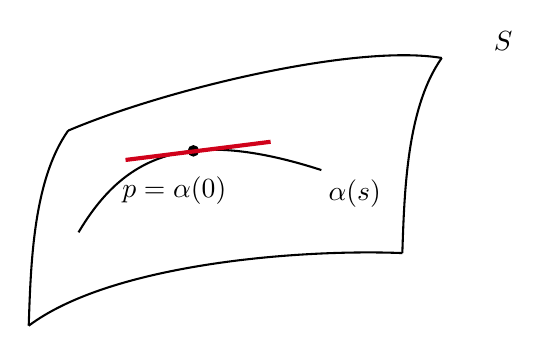
\begin{tikzpicture}[x=0.75pt,y=0.75pt,yscale=-1,xscale=1]
            %uncomment if require: \path (0,300); %set diagram left start at 0, and has height of 300

            %Curve Lines [id:da968109591651267] 
            \draw    (235.4,147.5) .. controls (282.4,127.5) and (374.4,105.5) .. (415.4,112.5) ;
            %Curve Lines [id:da9628832995393517] 
            \draw    (216.4,241.5) .. controls (256.4,211.5) and (347.4,204.5) .. (396.4,206.5) ;
            %Curve Lines [id:da9199503670863729] 
            \draw    (216.4,241.5) .. controls (217.4,212.5) and (218.4,171.5) .. (235.4,147.5) ;
            %Curve Lines [id:da1283058403662014] 
            \draw    (396.4,206.5) .. controls (397.4,177.5) and (398.4,136.5) .. (415.4,112.5) ;
            %Shape: Circle [id:dp20527443514441757] 
            \draw  [fill={rgb, 255:red, 0; green, 0; blue, 0 }  ,fill opacity=1 ] (293.5,157.25) .. controls (293.5,156.01) and (294.51,155) .. (295.75,155) .. controls (296.99,155) and (298,156.01) .. (298,157.25) .. controls (298,158.49) and (296.99,159.5) .. (295.75,159.5) .. controls (294.51,159.5) and (293.5,158.49) .. (293.5,157.25) -- cycle ;
            %Curve Lines [id:da8727495146013418] 
            \draw    (240.4,196.5) .. controls (262.4,159.5) and (292.4,145.5) .. (357.4,166.5) ;
            %Straight Lines [id:da5229930312194522] 
            \draw [color={rgb, 255:red, 208; green, 2; blue, 27 }  ,draw opacity=1 ][line width=1.5]    (263.05,161.63) -- (332.95,152.88) ;

            % Text Node
            \draw (439,98.4) node [anchor=north west][inner sep=0.75pt]    {$S$};
            % Text Node
            \draw (260,168.4) node [anchor=north west][inner sep=0.75pt]    {$p=\alpha ( 0)$};
            % Text Node
            \draw (359.4,169.9) node [anchor=north west][inner sep=0.75pt]    {$\alpha ( s)$};


        \end{tikzpicture}
    \end{center}
\end{definition}
\begin{definition}[Tangent space]
    \(T_p S={\text{all tangent vectors at p}}\).
    (\ie\ Tangent space is the collection of all tangent vectors of
    equivalent classes of curves passing through \(p\).)
\end{definition}
Here, we say two curves \(\alpha_1\colon(-\epsilon,\epsilon)\to S,
\alpha_2\colon(-\epsilon,\epsilon)\to S\) are equivalent at \(p\)
if \(\alpha_1(0)=\alpha_2(0)\) and \(\alpha_1'(0)=\alpha_2'(0)\).
\begin{center}



    \tikzset{every picture/.style={line width=0.75pt}} %set default line width to 0.75pt        

    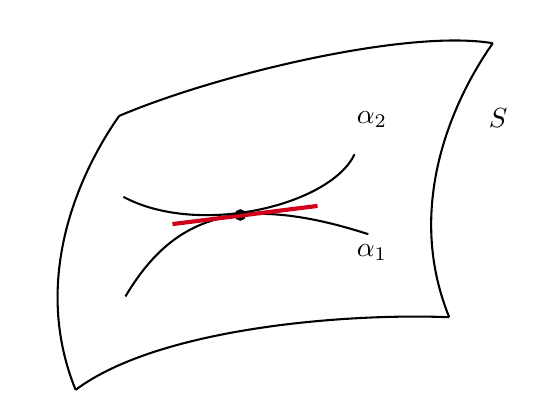
\begin{tikzpicture}[x=0.75pt,y=0.75pt,yscale=-1,xscale=1]
        %uncomment if require: \path (0,300); %set diagram left start at 0, and has height of 300

        %Curve Lines [id:da968109591651267] 
        \draw    (237.4,109.5) .. controls (284.4,89.5) and (376.4,67.5) .. (417.4,74.5) ;
        %Curve Lines [id:da9628832995393517] 
        \draw    (216.4,241.5) .. controls (256.4,211.5) and (347.4,204.5) .. (396.4,206.5) ;
        %Curve Lines [id:da9199503670863729] 
        \draw    (216.4,241.5) .. controls (193.8,186) and (220.4,133.5) .. (237.4,109.5) ;
        %Shape: Circle [id:dp20527443514441757] 
        \draw  [fill={rgb, 255:red, 0; green, 0; blue, 0 }  ,fill opacity=1 ] (293.5,157.25) .. controls (293.5,156.01) and (294.51,155) .. (295.75,155) .. controls (296.99,155) and (298,156.01) .. (298,157.25) .. controls (298,158.49) and (296.99,159.5) .. (295.75,159.5) .. controls (294.51,159.5) and (293.5,158.49) .. (293.5,157.25) -- cycle ;
        %Curve Lines [id:da8727495146013418] 
        \draw    (240.4,196.5) .. controls (262.4,159.5) and (292.4,145.5) .. (357.4,166.5) ;
        %Straight Lines [id:da5229930312194522] 
        \draw [color={rgb, 255:red, 208; green, 2; blue, 27 }  ,draw opacity=1 ][line width=1.5]    (263.05,161.63) -- (332.95,152.88) ;
        %Curve Lines [id:da5488316181309845] 
        \draw    (396.4,206.5) .. controls (373.8,151) and (400.4,98.5) .. (417.4,74.5) ;
        %Curve Lines [id:da7167451379981096] 
        \draw    (239.4,148.5) .. controls (275.8,168) and (339.2,152.5) .. (350.8,128) ;

        % Text Node
        \draw (414,104.4) node [anchor=north west][inner sep=0.75pt]    {$S$};
        % Text Node
        \draw (350.4,169.9) node [anchor=north west][inner sep=0.75pt]    {$\alpha _{1}$};
        % Text Node
        \draw (350.4,105.9) node [anchor=north west][inner sep=0.75pt]    {$\alpha _{2}$};


    \end{tikzpicture}
\end{center}
\begin{remark}
    \hfill
    \begin{enumerate}[(1)]
        \item This definition is sufficient in the following study of the
              course. Later, we will give another definition of tangent space
              by viewing a tangent vector as an operator acting on some equivalent
              class of \(C^\infty\) functions at a point.(\ie\ a tangent vector
              is a ``directional derivative'', which satisfies ``Linearity'' and
              ``Leibniz rule'') This will tell us how to take derivative of a
              function on a surface.
        \item In algebraic geometry course, you'll also see another
              definition of tangent vector (space) of an algebraic variety.
              You should make a comparison with these definitions, This is
              more abstract.
    \end{enumerate}
\end{remark}
\textbf{Claim:} Local expression of tangent vector is independent of the choice of
local param.
\begin{proof}
    Let \(\alpha(s)\colon (-\epsilon,\epsilon)\to S\) be the regular curve
    such that \(\alpha'(0)=V\) for the given tangent vector \(V\) at \(p\).
    Choose a local parametrization near \(p\),
    \begin{align*}
                     & F\colon  U\subset \mathbb{R}^2\to S \\
        (u,v)\mapsto & \left(x(u,v),y(u,v),z(u,v)\right)
        ,\end{align*}
    then \(\alpha(s)=\left(x\left(u(s),v(s)\right),y\left(u(s),v(s)\right),
    z\left(u(s),v(s)\right)\right)\). In fact, if we define
    \[
        \beta(s)=F^{-1}\circ\alpha(s)\colon (-\epsilon,\epsilon)\to U\subset
        \mathbb{R}^2
        ,\]
    then \(\alpha(s)=F\circ \beta (s)\).
    \begin{center}



        \tikzset{every picture/.style={line width=0.75pt}} %set default line width to 0.75pt        

        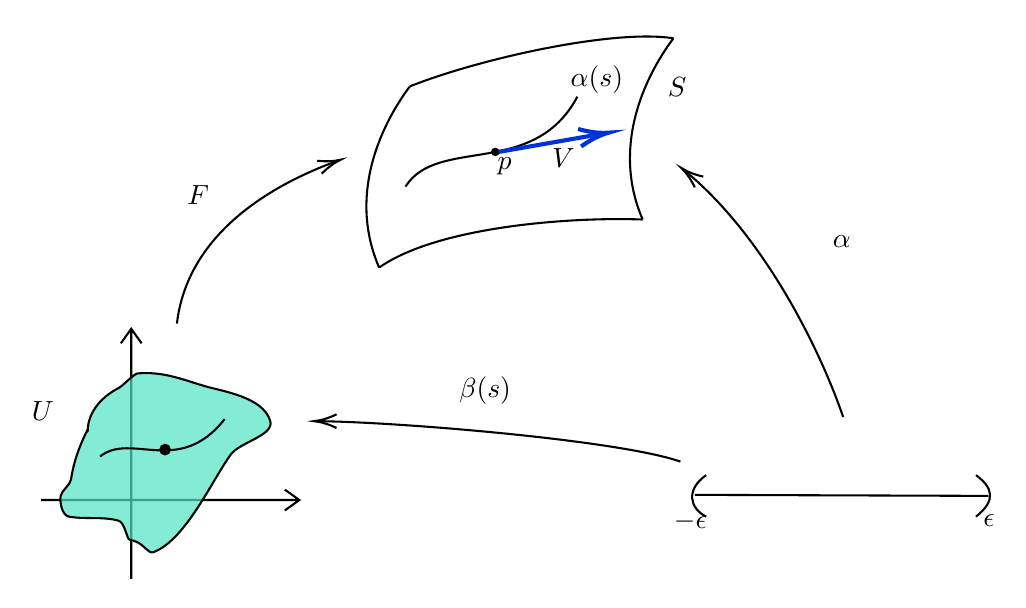
\begin{tikzpicture}[x=0.75pt,y=0.75pt,yscale=-1,xscale=1]
            %uncomment if require: \path (0,300); %set diagram left start at 0, and has height of 300

            %Curve Lines [id:da968109591651267] 
            \draw    (317.65,44.2) .. controls (350.81,30.97) and (415.7,16.42) .. (444.63,21.05) ;
            %Curve Lines [id:da9628832995393517] 
            \draw    (302.84,131.5) .. controls (331.05,111.66) and (395.25,107.03) .. (429.81,108.35) ;
            %Curve Lines [id:da9199503670863729] 
            \draw    (302.84,131.5) .. controls (286.89,94.79) and (305.66,60.07) .. (317.65,44.2) ;
            %Shape: Ellipse [id:dp20527443514441757] 
            \draw  [fill={rgb, 255:red, 0; green, 0; blue, 0 }  ,fill opacity=1 ] (357.22,75.78) .. controls (357.22,74.96) and (357.94,74.29) .. (358.81,74.29) .. controls (359.69,74.29) and (360.4,74.96) .. (360.4,75.78) .. controls (360.4,76.6) and (359.69,77.27) .. (358.81,77.27) .. controls (357.94,77.27) and (357.22,76.6) .. (357.22,75.78) -- cycle ;
            %Curve Lines [id:da8727495146013418] 
            \draw    (315.53,92.48) .. controls (331.05,68.01) and (377.19,88.84) .. (398.35,49.16) ;
            %Curve Lines [id:da5488316181309845] 
            \draw    (429.81,108.35) .. controls (413.87,71.65) and (432.64,36.92) .. (444.63,21.05) ;
            %Straight Lines [id:da7604427159074587] 
            \draw [color={rgb, 255:red, 0; green, 50; blue, 219 }  ,draw opacity=1 ][line width=1.5]    (360.4,75.78) -- (410.44,67.02) ;
            \draw [shift={(413.4,66.5)}, rotate = 170.07] [color={rgb, 255:red, 0; green, 50; blue, 219 }  ,draw opacity=1 ][line width=1.5]    (14.21,-4.28) .. controls (9.04,-1.82) and (4.3,-0.39) .. (0,0) .. controls (4.3,0.39) and (9.04,1.82) .. (14.21,4.28)   ;
            %Straight Lines [id:da8896542176151039] 
            \draw    (455,241) -- (596.4,241.5) ;
            %Curve Lines [id:da5641842523044696] 
            \draw    (460.4,231.5) .. controls (450.4,238.5) and (452.4,247.5) .. (460.4,251.5) ;
            %Curve Lines [id:da015954054171630094] 
            \draw    (590.4,231.5) .. controls (598.4,237.5) and (600.4,243.5) .. (590.4,251.5) ;
            %Curve Lines [id:da04574325182537042] 
            \draw    (526.4,203.5) .. controls (514.52,168.85) and (486.96,114.6) .. (449.54,84.41) ;
            \draw [shift={(448.4,83.5)}, rotate = 38.29] [color={rgb, 255:red, 0; green, 0; blue, 0 }  ][line width=0.75]    (10.93,-3.29) .. controls (6.95,-1.4) and (3.31,-0.3) .. (0,0) .. controls (3.31,0.3) and (6.95,1.4) .. (10.93,3.29)   ;
            %Shape: Axis 2D [id:dp9341218118059429] 
            \draw  (140,243.5) -- (264.4,243.5)(183.4,161) -- (183.4,281.5) (257.4,238.5) -- (264.4,243.5) -- (257.4,248.5) (178.4,168) -- (183.4,161) -- (188.4,168)  ;
            %Curve Lines [id:da5440535940443412] 
            \draw    (205.4,158.5) .. controls (210.32,116.14) and (249.21,92.22) .. (282.87,80.05) ;
            \draw [shift={(284.4,79.5)}, rotate = 160.56] [color={rgb, 255:red, 0; green, 0; blue, 0 }  ][line width=0.75]    (10.93,-3.29) .. controls (6.95,-1.4) and (3.31,-0.3) .. (0,0) .. controls (3.31,0.3) and (6.95,1.4) .. (10.93,3.29)   ;
            %Curve Lines [id:da3824738174976394] 
            \draw [fill={rgb, 255:red, 80; green, 227; blue, 194 }  ,fill opacity=0.7 ][line width=0.75] [line join = round][line cap = round]   (162.4,209.5) .. controls (158.54,217.23) and (155.61,225.06) .. (154.4,233.5) .. controls (153.99,236.38) and (149.97,238.65) .. (149.4,241.5) .. controls (148.84,244.32) and (149.93,250.87) .. (153.4,251.5) .. controls (160.88,252.86) and (170.14,251.32) .. (177.4,253.5) .. controls (180.16,254.33) and (181.45,262.26) .. (182.4,262.5) .. controls (188.34,263.98) and (188.09,265.27) .. (192.4,268.5) .. controls (192.93,268.9) and (193.78,268.75) .. (194.4,268.5) .. controls (209.81,262.34) and (222.3,234.01) .. (231.4,221.5) .. controls (235.62,215.7) and (252.35,212.33) .. (250.4,205.5) .. controls (247.02,193.68) and (226.82,191.06) .. (218.4,188.5) .. controls (207.25,185.11) and (198.45,181.5) .. (186.4,182.5) .. controls (184.71,182.64) and (179.2,188.6) .. (177.4,189.5) .. controls (170.45,192.98) and (162.4,200.22) .. (162.4,210.5) ;
            %Curve Lines [id:da19048774017798897] 
            \draw    (168.4,222.5) .. controls (183.4,210.5) and (206.4,232.5) .. (228.4,204.5) ;
            %Shape: Circle [id:dp7678024484359296] 
            \draw  [fill={rgb, 255:red, 0; green, 0; blue, 0 }  ,fill opacity=1 ] (197.4,219.2) .. controls (197.4,217.93) and (198.43,216.9) .. (199.7,216.9) .. controls (200.97,216.9) and (202,217.93) .. (202,219.2) .. controls (202,220.47) and (200.97,221.5) .. (199.7,221.5) .. controls (198.43,221.5) and (197.4,220.47) .. (197.4,219.2) -- cycle ;
            %Curve Lines [id:da9825567076006667] 
            \draw    (448,225) .. controls (418.84,214.66) and (310.71,205.77) .. (273.07,205.51) ;
            \draw [shift={(271.4,205.5)}, rotate = 360] [color={rgb, 255:red, 0; green, 0; blue, 0 }  ][line width=0.75]    (10.93,-3.29) .. controls (6.95,-1.4) and (3.31,-0.3) .. (0,0) .. controls (3.31,0.3) and (6.95,1.4) .. (10.93,3.29)   ;

            % Text Node
            \draw (440.46,38.25) node [anchor=north west][inner sep=0.75pt]    {$S$};
            % Text Node
            \draw (393.65,32.63) node [anchor=north west][inner sep=0.75pt]    {$\alpha ( s)$};
            % Text Node
            \draw (384.76,72.56) node [anchor=north west][inner sep=0.75pt]    {$V$};
            % Text Node
            \draw (358.46,76.94) node [anchor=north west][inner sep=0.75pt]    {$p$};
            % Text Node
            \draw (443.4,247.9) node [anchor=north west][inner sep=0.75pt]    {$-\epsilon $};
            % Text Node
            \draw (592.4,248.9) node [anchor=north west][inner sep=0.75pt]    {$\epsilon $};
            % Text Node
            \draw (520,114.4) node [anchor=north west][inner sep=0.75pt]    {$\alpha $};
            % Text Node
            \draw (209,90.4) node [anchor=north west][inner sep=0.75pt]    {$F$};
            % Text Node
            \draw (340,182.4) node [anchor=north west][inner sep=0.75pt]    {$\beta ( s)$};
            % Text Node
            \draw (134,194.4) node [anchor=north west][inner sep=0.75pt]    {$U$};


        \end{tikzpicture}
    \end{center}
    \begin{equation}
        V=\alpha'(0)=\left.\pdv{(x,y,z)}{(u,v)}
        \vdot \pdv{(u,v)}{s}\right|_{s=0}\tag{1}
        .\end{equation}
    Now, let \(G\) be another parametrization
    \begin{align*}
                               & G \colon V \to S \\
        (\alpha,\beta) \mapsto &
        \left(x\left(\alpha,\beta\right),y\left(\alpha,\beta\right),
        z\left(\alpha,\beta\right)\right).
    \end{align*}
    Let \(\gamma \colon (-\epsilon,\epsilon)\to V\) be \(\gamma(s)=G^{-1}
    \circ \alpha(s)\colon (-\epsilon,\epsilon)\to V\),
    then \(\alpha(s)=G\circ \gamma(s)\), and
    \begin{equation}
        \alpha'(0)=\left.\pdv{(x,y,z)}{(\alpha,\beta)}\vdot \pdv{(\alpha,\beta)}{s}\right|_{s=0}\tag{2}
        .\end{equation}
    (1) and (2) are essentially the same by the chain rule, \ie\
    \[
        \left.\pdv{(x,y,z)}{(u,v)}
        \vdot \pdv{(u,v)}{s}\right|_{s=0}
        =
        \pdv{(x,y,z)}{(\alpha,\beta)}\vdot
        \underbrace{\pdv{(\alpha,\beta)}{(u,v)}\vdot\pdv{(u,v)}{(\alpha,\beta)}}_{\text{identity matrix}}
        \vdot\left. \pdv{(\alpha,\beta)}{s}
        \right|_{s=0}
    \]
\end{proof}
\begin{proposition}
    Let \(F\colon U\subset \mathbb{R}^2\to S\) be a local parametrization near \(p\) with \(F(q)=p\), then \(dF_q\left(\mathbb{R}^2\right)=T_pS\).
\end{proposition}
\begin{proof}
    \hfill
    \begin{enumerate}[(1)]
        \item \(dF_q\left(\mathbb{R}^2\right)\subset T_p S\)

              \(\forall V\in \mathbb{R}^2\), let \(\beta(t)=q+t V\in \mathbb{R}
              ^2\), then \(\beta'(0)=v\). Let \(\alpha(t)=F\left(\beta(t)\right)
              \) is a \(C^\infty\)- curve passing through \(p\), and
              \[T_p S\ni \alpha'(0)=dF_q\left(\beta'(0)\right)=dF_q(V)\]
        \item \(T_p S\subset dF_q\left(\mathbb{R}^2\right)\)

              \(V\in T_p S\). \(\Rightarrow \exists \alpha(t)\colon (-\epsilon,
              \epsilon)\to S\) such that \(\alpha(0)=p\) and \(\alpha'(0)=V\).
              Let $\beta(t)=F^{-1}\left(\alpha(t)\right)$, then \(\alpha(t)=F
              \left(\beta(t)\right)\). We remark \(\beta(t)\) is a \(C^\infty\)
              -curve in \(\mathbb{R}^2\).(Because we have checked the transition
              function is \(C^\infty\) and \(F^{-1}\) comes from the composition
              of transition function) Thus,
              \[V=\alpha'(0)=dF_q\left(\beta'(0)\right)\in \mathrm{im}\,dF_q\]
    \end{enumerate}
\end{proof}
\begin{remark}
    \hfill
    \begin{enumerate}[(1)]
        \item \(T_p S\) is the full image of linear space under a linear map, thus \(T_pS\) is a linear space of dimension 2.
        \item \(dF_q\) is injective \(\Rightarrow\)\(F_u(q),F_v(q)\) are
              linearly independent, and they are tangent vectors of coordinate
              curve \(F(u,v_0)\) and \(F(u_0,v)\) at \((u_0,v_0)=q\),
              which implies that \(T_pS =\Span\left\{F_u(q),F_v(q)\right\}\).
        \item \(TS=\bigsqcup_{p\in S}T_p S=
              \left\{(p,V)|p\in S,V\in T_pS\right\}\).
              This set can be given a smooth coordinate covering, and is called
              the tangent bundle of \(S\), which is a 4-d smooth manifold. The
              projection
              \begin{align*}
                  \pi\colon TS\to S \\
                  (p,V)\mapsto p
              \end{align*}
              is \(C^\infty\)
    \end{enumerate}
\end{remark}
\subsection*{Tangent vector, tangent space, tangent bundle and tangent vector field}
\begin{enumerate}[(1)]
    \item On \(\mathbb{R}^n\).
    \begin{itemize}
        \item A vector is \(V=(v^1,v^2,\ldots,v^n)\).
        \item A standard basis is \(\{e_1,e_2,\ldots,e_n\}\), where 
        \(e_i=(0,\ldots,\mathop{1}\limits^{i^{th}},\ldots,0)\).\\
        \(\Rightarrow V=\sum_{i=1}^n v^i e_i\).
        \item \(f\) is smooth in \(\mathbb{R}^n\), the directional 
        derivative  along a vector \(v\) at \(p\) is 
        \[
            \left(D_V f\right)(p)=\langle\grad f,V\rangle_p
                =\sum_{i=1}^n v^i\left.\pdv{f}{x^i}\right|_p  
                =\left.\left(\sum_{i=1}^n v^i\pdv{x^i}\right)f\right|_p.
        \]
        Hence, we can identify \(e_i=\pdv{x^i}\) for \(i=1,2,\ldots,n\)
        and shall call \(\pdv{x^i}\) the coordinate vector (field).
        \[
            \Rightarrow V=\sum_{i=1}^n  v^i e_i=\sum_{i=1}^n v^i\pdv
            {x^i}.   
        \]
        \item Note in this way, we actually view a vector \(V\) as a 
        first order linear operator acting on smooth functions, \ie\ 
        for \(p\in \mathbb{R}^n\)
        \[
            V_p \colon  C^\infty\left(\mathbb{R}^n\right)\to \mathbb{R}
        ,\]
        \[ 
            f\mapsto  V(f)(p)=\left(D_V f\right)(p)=\left(v^i\pdv{f}{x^i}
            \right)(p)
        .\]
         Furthermore, this defines
         \[
            V\colon C^\infty\left(\mathbb{R}^n\right)\to 
            C^\infty\left(\mathbb{R}^n\right)   
         \]
         \[
            f\mapsto V(f)   
         .\]
        The operator \(V\) satisfies
        \[
            \begin{cases}
                (V+k W)f=V(f)+kW(f)&\text{(Linearity)}\\
                V(fg)=V(f)g +f V(g)&\text{(Leibniz rule)}
            \end{cases}    
        \]
    \end{itemize}
    \item \(S\) is a regular surface in \(\mathbb{R}^3\), \(p\in S\)
    \begin{itemize}
        \item \(C^\infty(S)={\text{all smooth functions on }S}\).
        \item We have defined \(V\in T_p S\), if \(\exists\) a smooth
        curve \(\alpha\colon (-\epsilon,\epsilon)\to S\) such that
        \(\alpha(t)=p\), \(\alpha'(0)=V\).
        \item To compute \(V\), we choose a local parametrization
        \begin{align*}
            F\colon U(\subset \mathbb{R}^2) &\longrightarrow S\subset \mathbb{R}^3\\
            (y^1,y^2) &\longmapsto (x^1,x^2,x^3)
        .\end{align*}
        \(\Rightarrow \alpha(s)=F\left(y^1(s),y^2(s)\right)\) (This is to 
        say we consider 
        \(\alpha\colon(-\epsilon,\epsilon)\to U
        \mathop{\longrightarrow }\limits^{F} S\)).
        \[
            \Rightarrow V=\alpha'(0)=\left.
            \left(
            \sum_{i=1}^2\pdv{x^1}{y^i}\dv{y^i}{s},
            \sum_{i=1}^2\pdv{x^2}{y^i}\dv{y^i}{s},
            \sum_{i=1}^2\pdv{x^3}{y^i}\dv{y^i}{s}
            \right)
            \right|_{p(s=0)}.
        \]
        Notice \(V\) is a vector in \(\mathbb{R}^3\), by using notation
        in (1)
        \[
            V_p=\sum_{\alpha=1}^3\left(\sum_{i=1}^2\pdv{x^\alpha}{y^i}
            \dv{y^i}{s}\right)\left. \pdv{x^\alpha}  \right|_p.
        \]
        Clearly, the linearity and Leibniz rule hold for the 
        \[
            V_p\colon C^\infty(S)\to \mathbb{R}    
        \]
        \[
            f\mapsto V_p(f)=\left(\left(\sum_{\alpha=1}^3 \sum_{i=1}
            ^2 \pdv{x^\alpha}{y^i}\dv{y^i}{s}\pdv{x^\alpha}\right)f\right)
            (p)   \tag{a} 
        .\]
        Note that during the lecture, we have shown
        \[
            T_pS=dF_{F^{-1}(p)}\left(\mathbb{R}^2\right)=\Span
            \left\{F_{y^1},F_{y^2}\right\}    .
        \]
        Moreover, 
        \[
            F_{y^i}=\sum_{\alpha=1}^3\pdv{x^\alpha}{y^i}\pdv
            {x^\alpha},
        \] 
        by using the notation in (1), and we can write
        \[
            F_{y^i}=\pdv{F}{y^i}=dF_{F^{-1}(p)}\left(\pdv{y^i}\right),
            ~i=1,2.
        \]
        \[
            \Rightarrow T_p S=\Span\left\{
                dF_{F^{-1}(p)}\left(\pdv{y^1}\right),
                dF_{F^{-1}(p)}\left(\pdv{y^2}\right)
            \right\}  ,
        \]
        since \(dF_{F^{-1}(p)}\colon \mathbb{R}^2\to T_p S\) is a linear
        isomorphism. By abusing notation here (actually not)
        \[
            T_p S=\Span \left\{\pdv{y^1},\pdv{y^2}\right\}    
        ,\]
        and 
        \[
            V_p (f)=\left(\sum_{i=1}^2\dv{y^i}{s}\pdv{y^i}\right)(f)(p)    
        .\]
        Hence,
        \[
            T_p S=\{\text{all tangent vectors }v\text{ at }p\}.    
        \]
    \end{itemize}
    \begin{remark}
        If \(M\) is a smooth manifold of dimension \(n\). By definition,
        \(M\) is a topological manifold (\ie\ Hausdorff + second countable 
        + locally Euclidean) that admits a smooth structure, which means 
        that \(\exists\) a covering \(\left\{(U_\alpha,\varphi_\alpha)
        \right\}_{\alpha\in \Lambda}\) of \(M\) such that
        \begin{itemize}
            \item \(\varphi_\alpha\colon U_\alpha\to \varphi
            \left(U_\alpha\right)\subset \mathbb{R}^n\) is a 
            homeomorphism.
            \item \(\varphi_\beta\circ \varphi_\alpha^{-1}\colon
            \varphi_\alpha\left(U_\alpha\cap U_\beta\right)
            \to \varphi_\beta\left(U_\alpha\cap U_\beta\right)
            \)
            is \(C^\infty\), \(\forall\alpha,\beta\) such that 
            \(U_\alpha\cap U_\beta\neq \emptyset\).
        \end{itemize}
        \begin{center}
            


\tikzset{every picture/.style={line width=0.75pt}} %set default line width to 0.75pt        

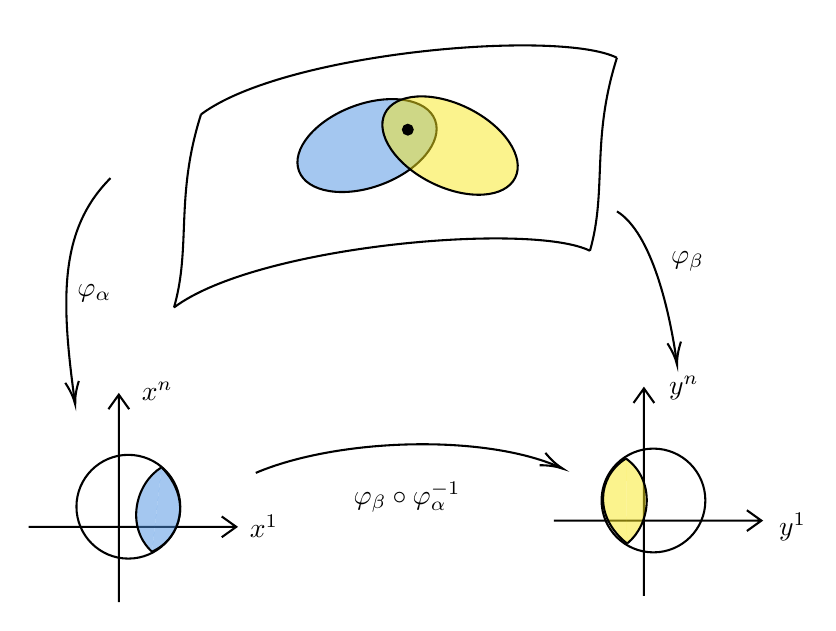
\begin{tikzpicture}[x=0.75pt,y=0.75pt,yscale=-1,xscale=1]
%uncomment if require: \path (0,300); %set diagram left start at 0, and has height of 300

%Curve Lines [id:da41714902560158285] 
\draw    (170,42) .. controls (210,12) and (342.4,0.7) .. (370.4,14.7) ;
%Curve Lines [id:da6592280103805965] 
\draw    (157,135) .. controls (197,105) and (329.4,93.7) .. (357.4,107.7) ;
%Curve Lines [id:da03942270080974852] 
\draw    (157,135) .. controls (165.4,105.7) and (157.4,81.7) .. (170,42) ;
%Curve Lines [id:da4108174147194943] 
\draw    (357.4,107.7) .. controls (365.8,78.4) and (357.8,54.4) .. (370.4,14.7) ;
%Shape: Ellipse [id:dp09147366462581186] 
\draw  [fill={rgb, 255:red, 74; green, 144; blue, 226 }  ,fill opacity=0.5 ] (217.21,69.25) .. controls (213.35,58.9) and (224.89,45.03) .. (243,38.26) .. controls (261.11,31.5) and (278.92,34.41) .. (282.79,44.75) .. controls (286.65,55.1) and (275.11,68.97) .. (257,75.74) .. controls (238.89,82.5) and (221.08,79.59) .. (217.21,69.25) -- cycle ;
%Shape: Ellipse [id:dp0011277621777061597] 
\draw  [fill={rgb, 255:red, 248; green, 231; blue, 28 }  ,fill opacity=0.5 ] (258.61,41.52) .. controls (263.49,31.61) and (281.51,30.51) .. (298.85,39.06) .. controls (316.18,47.61) and (326.28,62.57) .. (321.39,72.48) .. controls (316.51,82.39) and (298.49,83.49) .. (281.15,74.94) .. controls (263.82,66.39) and (253.72,51.43) .. (258.61,41.52) -- cycle ;
%Shape: Circle [id:dp9698509963450805] 
\draw  [fill={rgb, 255:red, 0; green, 0; blue, 0 }  ,fill opacity=1 ] (267.3,49.35) .. controls (267.3,48.05) and (268.35,47) .. (269.65,47) .. controls (270.95,47) and (272,48.05) .. (272,49.35) .. controls (272,50.65) and (270.95,51.7) .. (269.65,51.7) .. controls (268.35,51.7) and (267.3,50.65) .. (267.3,49.35) -- cycle ;
%Shape: Axis 2D [id:dp6551476919278265] 
\draw  (87,240.7) -- (187,240.7)(130.4,177) -- (130.4,277) (180,235.7) -- (187,240.7) -- (180,245.7) (125.4,184) -- (130.4,177) -- (135.4,184)  ;
%Shape: Circle [id:dp177276713898743] 
\draw   (110,231) .. controls (110,217.19) and (121.19,206) .. (135,206) .. controls (148.81,206) and (160,217.19) .. (160,231) .. controls (160,244.81) and (148.81,256) .. (135,256) .. controls (121.19,256) and (110,244.81) .. (110,231) -- cycle ;
%Curve Lines [id:da6569656679367748] 
\draw [fill={rgb, 255:red, 74; green, 144; blue, 226 }  ,fill opacity=0.5 ]   (151,212) .. controls (138.4,219.7) and (133.4,240.7) .. (146.4,252.7) ;
%Curve Lines [id:da7123507841915766] 
\draw [fill={rgb, 255:red, 74; green, 144; blue, 226 }  ,fill opacity=0.5 ]   (151,212) .. controls (165.4,226.7) and (161.4,245.7) .. (146.4,252.7) ;

%Shape: Axis 2D [id:dp8381858872649515] 
\draw  (340,237.7) -- (440,237.7)(383.4,174) -- (383.4,274) (433,232.7) -- (440,237.7) -- (433,242.7) (378.4,181) -- (383.4,174) -- (388.4,181)  ;
%Shape: Circle [id:dp1821947594932496] 
\draw   (363,228) .. controls (363,214.19) and (374.19,203) .. (388,203) .. controls (401.81,203) and (413,214.19) .. (413,228) .. controls (413,241.81) and (401.81,253) .. (388,253) .. controls (374.19,253) and (363,241.81) .. (363,228) -- cycle ;
%Curve Lines [id:da681192978192037] 
\draw [fill={rgb, 255:red, 248; green, 231; blue, 28 }  ,fill opacity=0.5 ]   (375.31,248.74) .. controls (386.84,239.52) and (389.15,218.05) .. (374.74,207.79) ;
%Curve Lines [id:da017656322535560598] 
\draw [fill={rgb, 255:red, 248; green, 231; blue, 28 }  ,fill opacity=0.5 ]   (375.31,248.74) .. controls (359.17,235.98) and (360.74,216.63) .. (374.74,207.79) ;

%Curve Lines [id:da09702567177122501] 
\draw    (370.4,88.7) .. controls (387.36,99.13) and (395.96,137.7) .. (399.16,160.94) ;
\draw [shift={(399.4,162.7)}, rotate = 262.57] [color={rgb, 255:red, 0; green, 0; blue, 0 }  ][line width=0.75]    (10.93,-3.29) .. controls (6.95,-1.4) and (3.31,-0.3) .. (0,0) .. controls (3.31,0.3) and (6.95,1.4) .. (10.93,3.29)   ;
%Curve Lines [id:da6721304677149988] 
\draw    (126.4,72.7) .. controls (101.65,97.45) and (102.38,131.02) .. (109.19,180.2) ;
\draw [shift={(109.4,181.7)}, rotate = 262.03] [color={rgb, 255:red, 0; green, 0; blue, 0 }  ][line width=0.75]    (10.93,-3.29) .. controls (6.95,-1.4) and (3.31,-0.3) .. (0,0) .. controls (3.31,0.3) and (6.95,1.4) .. (10.93,3.29)   ;
%Curve Lines [id:da9747233759845033] 
\draw    (196.4,214.7) .. controls (235.8,197.95) and (306.25,195.76) .. (342.76,211.95) ;
\draw [shift={(344.4,212.7)}, rotate = 205.28] [color={rgb, 255:red, 0; green, 0; blue, 0 }  ][line width=0.75]    (10.93,-3.29) .. controls (6.95,-1.4) and (3.31,-0.3) .. (0,0) .. controls (3.31,0.3) and (6.95,1.4) .. (10.93,3.29)   ;

% Text Node
\draw (395,106.4) node [anchor=north west][inner sep=0.75pt]    {$\varphi _{\beta }$};
% Text Node
\draw (109,122.4) node [anchor=north west][inner sep=0.75pt]    {$\varphi _{\alpha }$};
% Text Node
\draw (242,217.4) node [anchor=north west][inner sep=0.75pt]    {$\varphi _{\beta } \circ \varphi _{\alpha }^{-1}$};
% Text Node
\draw (192,233.4) node [anchor=north west][inner sep=0.75pt]    {$x^{1}$};
% Text Node
\draw (140,169.4) node [anchor=north west][inner sep=0.75pt]    {$x^{n}$};
% Text Node
\draw (447,232.4) node [anchor=north west][inner sep=0.75pt]    {$y^{1}$};
% Text Node
\draw (394,166.4) node [anchor=north west][inner sep=0.75pt]    {$y^{n}$};


\end{tikzpicture}
        \end{center}
        Note that \(\varphi_\alpha\colon U_\alpha \to \varphi_\alpha
        \left(U_\alpha\right)\) actually endow a coordinate on the chart
         \(U_\alpha\), \ie\ \(p\in U_\alpha\), \(\varphi_\alpha(p)
         =\left(x^1(p),x^2(p),\ldots,x^n(p)\right).
         \)
         Hence, \(p\in M\), choose \(U_\alpha\) as its coordinate chart
         \[
            \Rightarrow T_p M=\Span\left\{\pdv{x^1},\ldots,\pdv{x^n}
            \right\}.
         \]
         Note that if at \(p\), there are two coordinate charts
         \[
             \left\lbrace U,\left(x^1,\ldots,x^n\right)\right\rbrace
             \text{ and } 
             \left\lbrace V,\left(y^1,\ldots,y^n\right)\right\rbrace,
         \]
         and a vector \(V\in T_p S\) is expressed as 
         \[
            V=\sum_{i=1}^n V^i\pdv{x^i}=\sum_{\alpha=1}^n 
            \widetilde{V}^\alpha \pdv{y^\alpha}   
         ,\]
         then 
         \[
                \widetilde{V}^\alpha=V^i\pdv{y^\alpha}{x^i}
            \]
    \end{remark}
    \item Tangent (vector) bundle
    
    In (2), we have seen that the tangent space \(T_p S\) of a regular 
    surface does not depend on how we ``put'' \(S\) inside 
    \(\mathbb{R}^3\), and that \(T_p S=\Span\left\{\pdv{y^1},\pdv{y^2}
    \right\}\) for \(\left(y^1,y^2\right)\) a local coordinate in a 
    neighborhood of \(p\). This discussion holds for any smooth manifold.

    In the following, let's just give the general discussion.
    \begin{itemize}
        \item Let \(M\) be a smooth manifold, \(\forall p\in M\), 
        \(T_p M\) is the tangent space at \(p\). Define
        \[
            TM=\bigsqcup_{p\in M}T_p M=\left\{(p,V)| p\in M, V\in 
            T_p M\right\}   
        ,\]
        then there is a projection map 
        \[
            \pi\colon TM\to M
            \]
        \[
            (p,V)\mapsto p.      
            \]
        We shall show that the total space of \(TM\to M\) is a \(2n\)-dim
        smooth manifold such that \(\pi\colon TM \to M\) is a smooth map. 
        To achieve this goal, we need to define a smooth structure on the 
        total space \(TM\).
        \item \(M\) is a smooth manifold, by definition, \(\exists\) a
        countable covering \(\left\{\left(U\alpha,\varphi_\alpha\right)
        \right\}_{\alpha\in \Lambda}\) such that
        \begin{itemize}
            \item \(\varphi_\alpha\colon U_\alpha\to \varphi
            \left(U_\alpha\right)\subset \mathbb{R}^n\) is a 
            homeomorphism,
            \[
                \varphi_\alpha(p)=\left(x^1_\alpha(p),
                x^2_\alpha(p),\ldots,x^n_\alpha(p)\right).
            \]
            \item \(\varphi_\beta\circ \varphi_\alpha^{-1}\colon
            \varphi_\alpha\left(U_\alpha\cap U_\beta\right)
            \to \varphi_\beta\left(U_\alpha\cap U_\beta\right)
            \) is smooth, \(\forall\alpha,\beta\) such that 
            \(U_\alpha\cap U_\beta\neq \emptyset\).
        \end{itemize}
        \item For each \(U_\alpha\), \(\pi^{-1}\left(U_\alpha\right)\)
        contains all pairs \((p,V),p\in U_\alpha,V\in T_p M\). We define
        local trivialization (an local coordinate chart near \((p,V)\) 
        by letting 
        \[
            \widetilde{\varphi}_\alpha\colon 
            \pi^{-1}\left(U_\alpha\right)\to U_\alpha\times 
            \mathbb{R}^n
        \]
        \[
            (p,V)\mapsto \left(\varphi_\alpha(p),V^1,V^2,\ldots,
            V^n\right).    
        \]
        Note \(\widetilde{\varphi}_\alpha(p)=\left(x^1_\alpha(p)
        ,x^2_\alpha(p),\ldots,x^n_\alpha(p)\right)\), 
        \(V=\sum_{i=1}^n V^i(p)\pdv{x^i}\), then
        \[\widetilde{\varphi}_\alpha^{-1}\left(x^1_\alpha
        ,\ldots,x^n_\alpha;V^1,\ldots,V^n\right)=
        \left(p,\sum V^i \pdv{x^i}\right)
        ,\]
        \ie\ \(\widetilde{\varphi}_\alpha\) is bijective and
        \(\widetilde{\varphi}_\alpha\left(\pi^{-1}\left(
            U_\alpha
        \right)\right)\) is an open set.
        Then \(\left\{\widetilde{\varphi}_\alpha^{-1}\left(
            U_\alpha\times \mathbb{R}^n
        \right)\right\}_{\alpha\in \Lambda}\)
        is a countable covering of \(TM\).
        Moreover, this defines a topology on \(TM\), such that
        \[
            \widetilde{\varphi}_\alpha\colon \pi^{-1} 
            \left(U_\alpha\right) \to U_\alpha \times{R}^n  
        \]
        is a homeomorphism.
        Next, if \(\pi^{-1}\left(U_\alpha \right)\cap
        \pi^{-1}\left(U_\beta\right)\neq \emptyset\left(
            \Leftrightarrow U_\alpha\cap U_\beta\neq \emptyset
        \right)\), let \(p\in U_\alpha\cap U_\beta\)
        and 
        \[
            \widetilde{\varphi}_\alpha(p,V)
            = \left(x^1_\alpha(p),
            \cdots,x^n_\alpha(p);
            V^1_\alpha,\ldots,V^n_\alpha
            \right)
        \]
        \[
            \widetilde{\varphi}_\beta(p,V)
            = \left(x^1_\beta(p),
            \cdots,x^n_\beta(p);
            V^1_\beta,\ldots,V^n_\beta
            \right) 
        \]
        \begin{align*}
            \Rightarrow
            \widetilde{\varphi}_\beta\circ 
            \widetilde{\varphi}_\alpha^{-1}
            \left(
                x^1_\alpha(p),
            \cdots,x^n_\alpha(p);
            V^1_\alpha,\ldots,V^n_\alpha
            \right)
            \\=
            \left(x^1_\beta(p),
            \cdots,x^n_\beta(p);
            V^1_\beta,\ldots,V^n_\beta
            \right), 
        \end{align*}
            where
            \[
                V_p=\sum_{i=1}^n V^i_\alpha \pdv{x_\alpha^i}
                =\sum_{j=1}^n V^j_\beta\pdv{x_\beta^j}  
            \]
            \[
                V^j_\beta=\sum_{i=1}^n V^i_\alpha 
                \pdv{y^j_\beta}{x^i_\alpha}    
            ,\]
        \ie\ 
        \begin{align*}
            &\widetilde{\varphi}_\beta\circ 
            \widetilde{\varphi}_\alpha^{-1}
            \left(
                x^1_\alpha(p),
            \cdots,x^n_\alpha(p);
            V^1_\alpha,\ldots,V^n_\alpha
            \right)
            \\&=
            \left(
                \varphi_\beta\circ \varphi_\alpha^{-1}
                \left(x^1_\alpha,\ldots,x^n_\alpha\right);
                \sum_{i=1}^n V^i_\alpha 
                \pdv{y^1_\beta}{x^i_\alpha},
                \cdots,
                \sum_{i=1}^n V^i_\alpha 
                \pdv{y^n_\beta}{x^i_\alpha}
            \right)
        .\end{align*}
        Hence, \(\widetilde{\varphi}_\beta\circ 
        \widetilde{\varphi}_\alpha^{-1}\) is smooth since 
        \(\varphi_\beta\circ \varphi_\alpha^{-1}\)
        is smooth, and the transition function on the vector part 
        is just linear.
        \item The Hausdorff property of \(TM\) is also clear from 
        the Hausdorff property of \(M\).
        \item With the smooth structure defined above, Clearly
        \(\pi\colon TM\to M\) is a smooth map since \(\pi\) is
        just a projection (when expressed in coordinate).
    \end{itemize}
\end{enumerate}
    \textbf{Tangent vector field}
        
\begin{definition}
            A smooth vector field \(V\) is a \(C^\infty\)-map
            \[
                V\colon M\to TM    
            \]
            such that \(\pi\circ V=\mathrm{id}_M\). In a coordinate
            chart \(\left(U_\alpha,\left(x^1_\alpha,\ldots
            x^n_\alpha
            \right)\right)\), \[
              V=\sum_{i=1}^n V^i_\alpha(x)\pdv{x^i_\alpha} 
            \]
\end{definition}
\begin{remark}
            \hfill
        \begin{enumerate}[(1)]
                \item A smooth vector field is also called a smooth
                section of the tangent (vector) bundle.
                \item Since the tangent vector is linear and satisfies
                the Leibniz rule, so is the vector field. Hence,
                \[
                    V\colon C^\infty(M)\to C^\infty(M)    
                \]
                \[
                    f\mapsto V(f)    
                \]
                is characterized by 
                \(V(fg)=V(f)g+fV(g)\).
        \end{enumerate}
\end{remark}
\begin{exercise}
    \hfill
    \begin{enumerate}[(1)]
        \item \(\mathbb{S}^1\): unit circle. 
        \(T\mathbb{S}^1\simeq \mathbb{S}^1 \times \mathbb{R}\) 
        is a diffeomorphism.
        
        Intuitive observation of this diffeomorphism: we can
        choose local charts on \(\mathbb{S}^1\) by 
        \[\theta\in (0,2\pi)=U, ~\varphi \in 
        (\frac{\pi}{2},\frac{3\pi}{2})=V\]
        \ie\ \(\varphi=\theta+\frac{\pi}{2}\), which is simply
        a rotation. 
        \[\left.T\mathbb{S}^1\right|_U=\left\{
            \left(\theta,a(\theta)\pdv{\theta}\right)
        \right\}\]
        \[
            \left.T\mathbb{S}^1\right|_V=\left\{
            \left(\varphi,a(\varphi)\pdv{\varphi}\right)
            \right\}   
        .\]
        In this case, 
        the transition function is just linear by rotation.
        Hence, \(\left.T\mathbb{S}^1\right|_U\) and 
        \(\left.T\mathbb{S}^1\right|_V\) can be glued by shifting 
        \(\frac{\pi}{2}\).
        \item \(\mathbb{S}^2\) unit sphere.
        However, \(T\mathbb{S}^2\ncong \mathbb{S}^2\times 
        \mathbb{R}^2\).
        To see this, we take stereographical parametrization.
        (Since there are only two coordinate charts)
        \begin{align*}
            p_N\colon &\mathbb{S}^2-\{N\}\to \mathbb{R}^2\\
            (x,y,z)&\mapsto \left(\frac{x}{1-z},\frac{y}{1-z}\right)    
        \end{align*}
        \begin{align*}
            p_S\colon &\mathbb{S}^2-\{S\}\to \mathbb{R}^2\\
            (x,y,z)&\mapsto \left(\frac{y}{1+z},\frac{x}{1+z}\right)    
        .\end{align*}
        The transition function is given by 
        \[
          p_S\circ p_N^{-1}(x,y)=\left(\frac{y}{x^2+y^2},
          \frac{x}{x^2+y^2}\right)=(u,v)  
        \]
        \[
            \Rightarrow
            \begin{cases}
                \pdv{x}=-2uv\pdv{u}+\left(v^2-u^2\right)\pdv{v}\\
                \pdv y= \left(u^2-v^2\right)\pdv{u}
                -2uv\pdv{v}
            \end{cases}    
        .\]  
        Note \((x,y)=(0,0)\) is just the north pole and 
        \((u,v)=(0,0)\) is just the south pole. 
        At these two points, the coordinate vector fields 
        are zero vectors, e.g. \(\pdv{x},\pdv{y}\) are zero
        vectors at the south pole.
        This means that we can not extend the tangent 
        plane in the trivialization 
        \(p_N^{-1}\left(\mathbb{R}^2\right)\)
        passing through the south pole, hence we can not
        have a global trivialization of \(T\mathbb{S}^2\).
         \(T\mathbb{S}^2\ncong \mathbb{S}^2\times 
         \mathbb{R}^2\)
    \end{enumerate}         
\end{exercise}
Next, we would like to mention a more abstract way to think 
about the tangent space.
\begin{itemize}
    \item \(M\) is a smooth manifold, \(p\in M\)
    \item \(C_p^\infty(M)\)=\{all \(C^\infty\) functions
    on \(M\) vanishing at \(p\)\}.\\
    \(C_p^\infty(M)^2\)=\{all finite sums 
    \(\sum f_i g_i \) with \(f_i,g_i\in C_p^\infty(M)\)\}
    \[
        \Rightarrow C^\infty(M)=
        \left\{\text{constant functions}\right\}\oplus 
        C^\infty_p(M)=\mathbb{R}\oplus C^\infty_p(M).     
    \]
    \item Let \(V\) be an tangent vector at \(p\), 
    \(V\colon C^\infty(M)\to \mathbb{R}\) and \(V|_{\mathbb{R}}=0\).
    Moreover, it's easy to see by the Leibniz rule that 
    \(V|_{C_p^\infty(M)^2}=0\)
    \[
          \Rightarrow V\colon C_p^\infty(M)/C_p^\infty(M)^2
          \to \mathbb{R}
    \]
    is a linear map, \ie\ \(V\in 
    \left(C_p^\infty(M)/C_p^\infty(M)^2\right)^*\)

    \(\Rightarrow T_p M\simeq 
    \left(C_p^\infty(M)/C_p^\infty(M)^2\right)^*\)
    is an isomorphism. Hence, we can define tangent space
    \(T_p M\) as 
    \(\left(C_p^\infty(M)/C_p^\infty(M)^2\right)^*\)

    This definition tells that a tangent vector is a linear map 
    on \(C^\infty(M)\) vanishing on constants and only depends 
    on the first order Taylor's expansion of a function \(f\)
    at \(p\).

    In algebraic geometry language, the vanishing ideals 
    \(C^\infty_p(M)\) are the maximal ideals in the algebra
     of smooth functions, with \(C_p^\infty(M)^2\) the second
     power. More generally, for any maximal ideal \(I\) in a 
     commutative algebra \(A\), one may define the tangent space as 
    \(\left(I/I^2\right)^*\).
\end{itemize}
\begin{remark}
    This last part is not required in this course.
\end{remark}
